% !TEX program = xelatex
% !TEX encoding = UTF-8 Unicode
%=============================================================================
%  대한조선학회논문집 (Journal of the Society of Naval Architects of Korea)
%  투고 양식  —  "논문작성양식(한글) (2).hwp" 의 서식을 그대로 옮긴 LaTeX 판본
%
%  용지   : A4 210 x 297 mm
%           여백 좌/우 20 mm, 위 25 mm(머리말 8 mm), 아래 15 mm(꼬리말 7 mm)
%           → 판면 170 x 242 mm, 본문 시작 33 mm
%  단     : 2단, 단 간격 8 mm (단 폭 81 mm)
%  글꼴   : 한글 한컴돋움 / 영문 돋움체
%           국문제목 20 pt · 국문저자 12 pt · 영문제목 18 pt · 영문저자 12 pt
%           요약 13 pt B · 초록본문 10 pt · Keywords 9 pt
%           장제목 15 pt B(가운데) · 절제목 11 pt(가운데) · 본문 9.5 pt
%           표/그림 캡션 10 pt · 표 내용 9 pt · 안내문 8 pt
%  들여쓰기 : 본문 첫 줄 +7.1 mm, 참고문헌 내어쓰기 -7.1 mm
%
%  컴파일 : xelatex SNAK_paper_template.tex   (2회 실행)
%=============================================================================
\documentclass[10pt,twocolumn]{extarticle}

%----------------------------------------------------------------- 용지·판면
\usepackage[
  papersize={210mm,297mm},
  left=20mm, right=20mm,
  top=33mm,  bottom=22mm,     % 위 25 + 머리말 8 / 아래 15 + 꼬리말 7
  columnsep=8mm
]{geometry}

%----------------------------------------------------------------- 한글 글꼴
\usepackage{kotex}
\usepackage{fontspec}

%-----------------------------------------------------------------------------
%  HWP 문자모양은 "한글 글꼴"과 "영문 글꼴"을 따로 지정합니다.
%  이 양식은 한글 = 한컴돋움, 영문 = 돋움체 로 지정되어 있습니다.
%
%    HWP 지정      LaTeX 사용        비고
%    ----------    --------------    ----------------------------------------
%    한컴돋움      Haansoft Dotum    원본 그대로 (HDOTUM.TTF)
%    돋움체        DotumChe          원본 그대로
%    굴림          Gulim             원본 그대로
%
%  한컴돋움(Haansoft Dotum)은 한컴오피스에 포함된 글꼴입니다. XeTeX(fontconfig)이
%  인식하려면 C:\Windows\Fonts 또는 TeX Live 글꼴 트리에 있어야 하므로, 이 PC 에는
%    C:\texlive\2026\texmf-dist\fonts\truetype\hancom\HDOTUM.TTF
%  로 설치(원본: 한컴오피스 ...\HOffice120\Shared\TTF\All\HDOTUM.TTF)한 뒤
%  fc-cache -f 를 실행해 두었습니다.
%
%  한컴돋움이 없는 PC 에서는 아래 \BodyHangulFont 를 {HCR Dotum}(함초롬돋움)
%  으로 바꾸면 컴파일됩니다. (자폭이 0.97 em 이라 줄바꿈이 원본과 달라집니다.)
%-----------------------------------------------------------------------------
\def\BodyHangulFont{Haansoft Dotum}  % 한컴돋움
\def\LatinFont{DotumChe}             % 돋움체 (모든 영문)

%  HWP 문자모양의 글자 폭 설정 (이 양식은 거의 모든 문자모양이 동일)
%    장평(자폭 비율) = 93 %   →  FakeStretch=0.93   (가로로만 93 % 축소)
%    자간            = -12 %  →  한글: InterHangul=-0.12em
%                                영문: LetterSpace=-12.0
%  주의: fontspec 의 LetterSpace 는 한글 글자 사이에는 적용되지 않는다
%        (어절 공백에만 먹는다). 한글 자간은 반드시 xetexko 의 InterHangul 을 쓸 것.
% DotumChe/한컴돋움에는 이탤릭 자형이 없다. AutoFakeSlant 를 주지 않으면
% 참고문헌의 \textit{저널명} 이 정체로 떨어진다(log: TU/DotumChe(0)/m/it undefined).
\setmainfont{\LatinFont}[Ligatures=TeX, AutoFakeBold=2.5, AutoFakeSlant=0.2,
                         FakeStretch=0.93, LetterSpace=-12.0]
\setmainhangulfont{\BodyHangulFont}[AutoFakeBold=2.5, AutoFakeSlant=0.2,
                         FakeStretch=0.93, InterHangul=-0.12em]
\setsanshangulfont{\BodyHangulFont}[AutoFakeBold=2.5, AutoFakeSlant=0.2,
                         FakeStretch=0.93, InterHangul=-0.12em]

% 초록(요약)만 영문 자간이 -8 % 이다 (HWP 문자모양 cs4). 본문은 -12 %.
\newfontfamily\AbstractLatin{\LatinFont}[Ligatures=TeX, AutoFakeBold=2.5,
                         FakeStretch=0.93, LetterSpace=-8.0]

%----------------------------------------------------------------- 기타 패키지
\usepackage[fleqn]{amsmath}
\usepackage{amssymb}
\usepackage{graphicx}
\usepackage{xcolor}
\usepackage{titlesec}
\usepackage{caption}
\usepackage{float}
\usepackage{array}
\usepackage{setspace}
\usepackage{textcomp}

\definecolor{snakred}{RGB}{255,0,0}
\definecolor{snakblue}{RGB}{0,0,255}
\newcommand{\guide}[1]{\textcolor{snakred}{#1}}   % 양식 안내문(빨강)

\graphicspath{{figs_snak/}}

%----------------------------------------------------------------- 본문 조판
% 행송(줄간격)은 아래 각 매크로에서 \fontsize{크기}{행송} 으로 직접 지정한다.
\renewcommand{\baselinestretch}{1}
\setlength{\parskip}{0pt}
\setlength{\columnsep}{8mm}

% 본문 : 9.5 pt, 줄간격 150 % (= 14.25 pt), 첫 줄 들여쓰기 7.1 mm
\renewcommand{\normalsize}{\fontsize{9.5}{14.25}\selectfont
  \abovedisplayskip 6pt plus 2pt minus 2pt
  \belowdisplayskip 6pt plus 2pt minus 2pt
  \abovedisplayshortskip 0pt plus 2pt
  \belowdisplayshortskip 4pt plus 2pt minus 2pt}
\normalsize
% 첫 줄 들여쓰기 = 1 글자(9.5 pt = 3.35 mm).
% HWP 문단모양의 indent 필드값(2000)을 그대로 환산하면 7.06 mm 가 되지만,
% 실제 조판 결과를 미리보기에서 실측하면 4개 문단 모두 3.48 mm(= 1 글자 + 좌측
% 사이드베어링)였다. 실측값을 따른다.
\setlength{\parindent}{9.5pt}

% HWP 는 마침표 뒤에 문장 간격을 더 주지 않는다 — 모든 공백을 동일하게
\frenchspacing

% HWP 는 영문 자동 하이픈을 넣지 않는다 — 동일하게 끔
\hyphenpenalty=10000
\exhyphenpenalty=10000
\tolerance=3000
\emergencystretch=1em
\raggedbottom

% 어절 사이 공백을 고정한다.
% FakeStretch(0.93) 와 LetterSpace(-12) 가 공백 폭까지 깎아 버려서 그대로 두면
% 1/3 em 보다 훨씬 좁아지고, 줄당 글자 수가 원본보다 많아진다.
% 아래 값은 HWP 원본 미리보기의 서론 문단 줄바꿈과 대조하며 맞춘 값이다.
\spaceskip=0.330em plus 0.090em minus 0.040em
\xspaceskip=0.330em plus 0.090em minus 0.040em

% xetexko 는 기본적으로 한글 글자 사이마다 plus.04em minus.02em 신축 글루를 넣는다.
% 그 때문에 줄을 꽉 채우지 않아도 벌점이 없어 원본보다 헐겁게 끊긴다.
% HWP 는 양쪽정렬 시 '어절 공백'만 늘리고 글자 피치는 고정이다(미리보기 실측:
% 자연 공백 1.45 mm → 정렬 후 1.74 mm, 글자 피치 불변). 그래서 0 으로 둔다.
\xetexkostretchshrink{plus0em minus0em}

\setlength{\mathindent}{5mm}    % 수식은 왼쪽 정렬(번호는 오른쪽)

\pagestyle{empty}               % 양식에 머리말·쪽번호 없음

%----------------------------------------------------------------- 장·절 제목
% 1. 서 론 / 2. ... : 15 pt B, 가운데
\renewcommand{\thesection}{\arabic{section}}
\renewcommand{\thesubsection}{\arabic{section}.\arabic{subsection}}

\titleformat{\section}[block]
  {\centering\bfseries\fontsize{15}{22.5}\selectfont}
  {\thesection.}{0.4em}{}
% 별표 없는 \titlespacing 을 써야 제목 다음 문단도 들여쓰기(7.1 mm)가 유지된다.
\titlespacing{\section}{0pt}{14.3pt plus 3pt minus 2pt}{12.7pt plus 1pt}

% 3.1 표의 예 : 11 pt(굵기 없음), 가운데
\titleformat{\subsection}[block]
  {\centering\fontsize{11}{16.5}\selectfont}
  {\thesubsection}{0.5em}{}
\titlespacing{\subsection}{0pt}{10pt plus 2pt}{5pt plus 1pt}

\titleformat{\subsubsection}[block]
  {\fontsize{10}{15}\selectfont}
  {\thesubsubsection}{0.5em}{}
\titlespacing*{\subsubsection}{0pt}{8pt plus 1pt}{4pt}

%----------------------------------------------------------------- 표·그림 캡션
% Table 캡션은 표 위·왼쪽 정렬,  Fig. 캡션은 그림 아래·가운데 정렬. 모두 10 pt
\DeclareCaptionFont{snakcap}{\fontsize{10}{13}\selectfont}
\captionsetup[table]{name=Table, labelsep=space, font=snakcap,
                     justification=raggedright, singlelinecheck=false,
                     skip=3pt, position=above}
\captionsetup[figure]{name=Fig., labelsep=space, font=snakcap,
                      justification=centering, singlelinecheck=false,
                      skip=4pt, position=below}

\renewcommand{\arraystretch}{1.4}

%----------------------------------------------------------------- 표제부 매크로
\newcommand{\KoreanTitle}[1]{{\centering\fontsize{20}{26}\selectfont #1\par}}
\newcommand{\KoreanAuthor}[1]{{\centering\fontsize{12}{18.7}\selectfont #1\par}}
\newcommand{\EnglishTitle}[1]{{\centering\fontsize{18}{23.4}\selectfont #1\par}}
\newcommand{\EnglishAuthor}[1]{{\centering\fontsize{12}{19.0}\selectfont #1\par}}
\newcommand{\AbstractHead}[1]{{\centering\bfseries\fontsize{13}{19.5}\selectfont #1\par}}

% 초록 본문 : 10 pt, 줄간격 130 %, 첫 줄 들여쓰기 7.1 mm
\newenvironment{snakabstract}
  {\par\AbstractLatin\fontsize{10}{13}\selectfont\setlength{\parindent}{7.1mm}}
  {\par}

% Keywords : 9 pt, 라벨 굵게(검정) + 내용 빨강
\newcommand{\snakkeywords}[1]{%
  \par\fontsize{9}{13.5}\selectfont\setlength{\parindent}{0pt}
  \noindent{\bfseries Keywords} : \guide{#1}\par}

% 양식 안내 블록 (8.5 pt B 제목 + 8 pt 본문, 모두 빨강)
\newenvironment{snakguide}[1]
  {\par\vspace{4pt}\color{snakred}\setlength{\parindent}{0pt}
   {\bfseries\fontsize{8.5}{12.75}\selectfont #1\par}
   \fontsize{8}{12}\selectfont}
  {\par\vspace{2pt}}

% 참고문헌 : 9.5 pt, 내어쓰기 7.1 mm
\newenvironment{snakreferences}
  {\par{\centering\fontsize{15}{22.5}\selectfont 참 고 문 헌\par}\vspace{6pt}%
   \fontsize{9.5}{14.25}\selectfont
   \setlength{\parindent}{-7.1mm}\setlength{\leftskip}{7.1mm}}
  {\par}

%=============================================================================

%=============================================================================

%=============================================================================
%  ※ 사실성 원칙 (MDFold/PAPER_PROMPT.md A.3, paper_prompt_llm_task_allocation.md §4)
%    - 본문의 모든 수치는 두 브리프(Part B/C, §2)에서만 가져온다.
%    - 미측정 항목은 [TODO]로 남기고 결과를 창작하지 않는다.
%    - 실재 확신 없는 인용은 [인용 필요: 주제]로 남긴다.
%=============================================================================
\begin{document}

\twocolumn[
\begin{@twocolumnfalse}
\vspace*{7.06mm}

\KoreanTitle{자폭 무인수상정 군집 방어를 위한 LLM 기반 임무배정과\\
점수맵 기반 다중 에이전트 방어 체계 구축}

\KoreanAuthor{윤영준(충남대학교), 방현태(충남대학교), 전유라(한국과학기술원), 김덕환(한국과학기술원), 윤원근(충남대학교)}

\vspace{7.75mm}

\EnglishTitle{LLM-Based Task Allocation and Score-Map\\
Reinforcement Learning for a Multi-Agent Defense\\
System against Suicide USV Swarms}

\EnglishAuthor{Yeongjun Yoon(Chungnam National Univ.), Hyeontaek Bang(Chungnam National Univ.), Yura Jeon(Korea Advanced Institute of Science and Technology), Deokhwan Kim(Korea Advanced Institute of Science and Technology), Wonkeun Youn(Chungnam National Univ.)}

\vspace{9.2mm}

\AbstractHead{요 약}

\vspace{10.5mm}

\begin{snakabstract}
Swarms of low-cost suicide unmanned surface vehicles (USVs) are difficult to
counter by conventional means: soft-kill jamming is indiscriminate, leaves the
warhead intact, and does not reach fiber-optic guided craft, while hard-kill
interceptors cost far more than the targets they destroy and engage them one at
a time. This paper therefore adopts physical capture, in which a small number of
defending USVs, slower than the attackers, deploy capture nets across the
approach corridors of a mothership. The defense is organized in two layers that
run on different decision cycles. A large language model (LLM) commander
receives a battlefield state whose geometry has already been computed, and
decides which enemy each vessel engages and which vessel holds; no combinatorial
optimizer revises that decision. The commander is called asynchronously, so its
response latency does not stall the control loop. Between successive replans the
battlefield is rasterized into a multi-channel image centred on the mothership,
and a parameter-shared convolutional policy turns that image into a score map
over the sea surface. Each vessel picks two high-scoring pixels within the
region assigned to it, and lays a net along the segment joining them. Picking
pixels on a score map, rather than regressing continuous waypoints, constrains
the action space and fixes the selected waypoints, keeping the maneuver stable.
\end{snakabstract}

\vspace{7.3mm}

\snakkeywords{Unmanned surface vehicle(무인수상정),
Swarm defense(군집 방어), Multi-agent reinforcement learning(다중 에이전트 강화학습),
Task allocation(임무배정), Large language model(대규모 언어모델),
Convolutional neural network(합성곱 신경망)}

\vspace{16mm}

\end{@twocolumnfalse}
]

%=============================================================================
\section{서 론}

%=============================================================================
%  도판 6종 — 생성 프롬프트는 「논문 그림/prompts/」 에 있다.
%    fig1_concept.png      교전 개념            \label{fig:concept}      단단
%    fig2_architecture.png 2계층 구조·비동기    \label{fig:architecture} 양단
%    fig3_commander.png    지휘관 계층          \label{fig:commander}    단단
%    fig4_observation.png  다채널 래스터 관측   \label{fig:observation}  단단
%    fig5_policy.png       점수맵 정책(U-Net)   \label{fig:policy}       양단
%    fig6_grpo.png         그룹상대 학습        \label{fig:grpo}         단단
%  파일은 figs_snak/ 에 넣는다(\graphicspath). 번호는 \begin{figure} 선언 순서를
%  따르므로 아래 순서를 바꾸면 Fig. 번호가 어긋난다.
%=============================================================================

다수의 저비용 무인수상정(Unmanned Surface Vehicle, USV)이 고가치 함정 한 척에게 여러
방향에서 동시에 돌진하는 자폭 공격은 대표적인 비대칭 전력이다. 유한한 아군 자산을 다수
표적에 배분하는 문제는 무기-표적 할당(weapon-target assignment)으로 연구되어
왔으나(Ahuja et al., 2007), 표적 수가 요격 자산을 넘어서면 최적 할당으로도 처리되지 않는
표적이 남는다.

무인 위협에 대한 기존 대응은 두 갈래로 구분된다(Wang et al., 2021). 표적의
통신·항법·센서를 교란하는 연성 대응(soft-kill)은 위협 자체를 제거하지 못하고, 전파를
방사하지 않는 유선 조종 표적에는 작용하지 않는다(Sutea, 2026). 표적을 직접 타격하는 경성 대응(hard-kill)은 위협을 확실히
제거하지만, 수천 달러 규모의 표적에 발당 수십만에서 수백만 달러의 요격 유도탄을
소모하는 비용 구조를 지탱하기 어렵다(Rumbaugh, 2024). 또한 한 번에 한 표적만 처리하므로
표적 수가 교전 용량을 넘어서면 포화가 발생한다.

본 연구는 대안으로 저비용 그물을 이용한 물리적 포획을 채택한다. 이는 무인기 대응
분야에서 독립된 대응 범주로 다루어져 왔으며(Wang et al., 2021), 표적의 통신 방식과
무관하게 작용하고 표적을 정지시킨다는 점에서 앞의 두 한계를 비켜간다. 소수의 방어정이
적선의 공격 경로를 예측하여 기동하며 투하한 그물이 적선의 추진기에 얽히며 
무력화시킨다. 그물은 유도탄보다 단가가 낮고 하드웨어적으로 적선을 무력화하므로, 다수의 표적을 경제적이고, 확실하게 처리할 수 있다.

%-------------------------------------------------- 그림 1 (단단)
\begin{figure}[H]
\centering
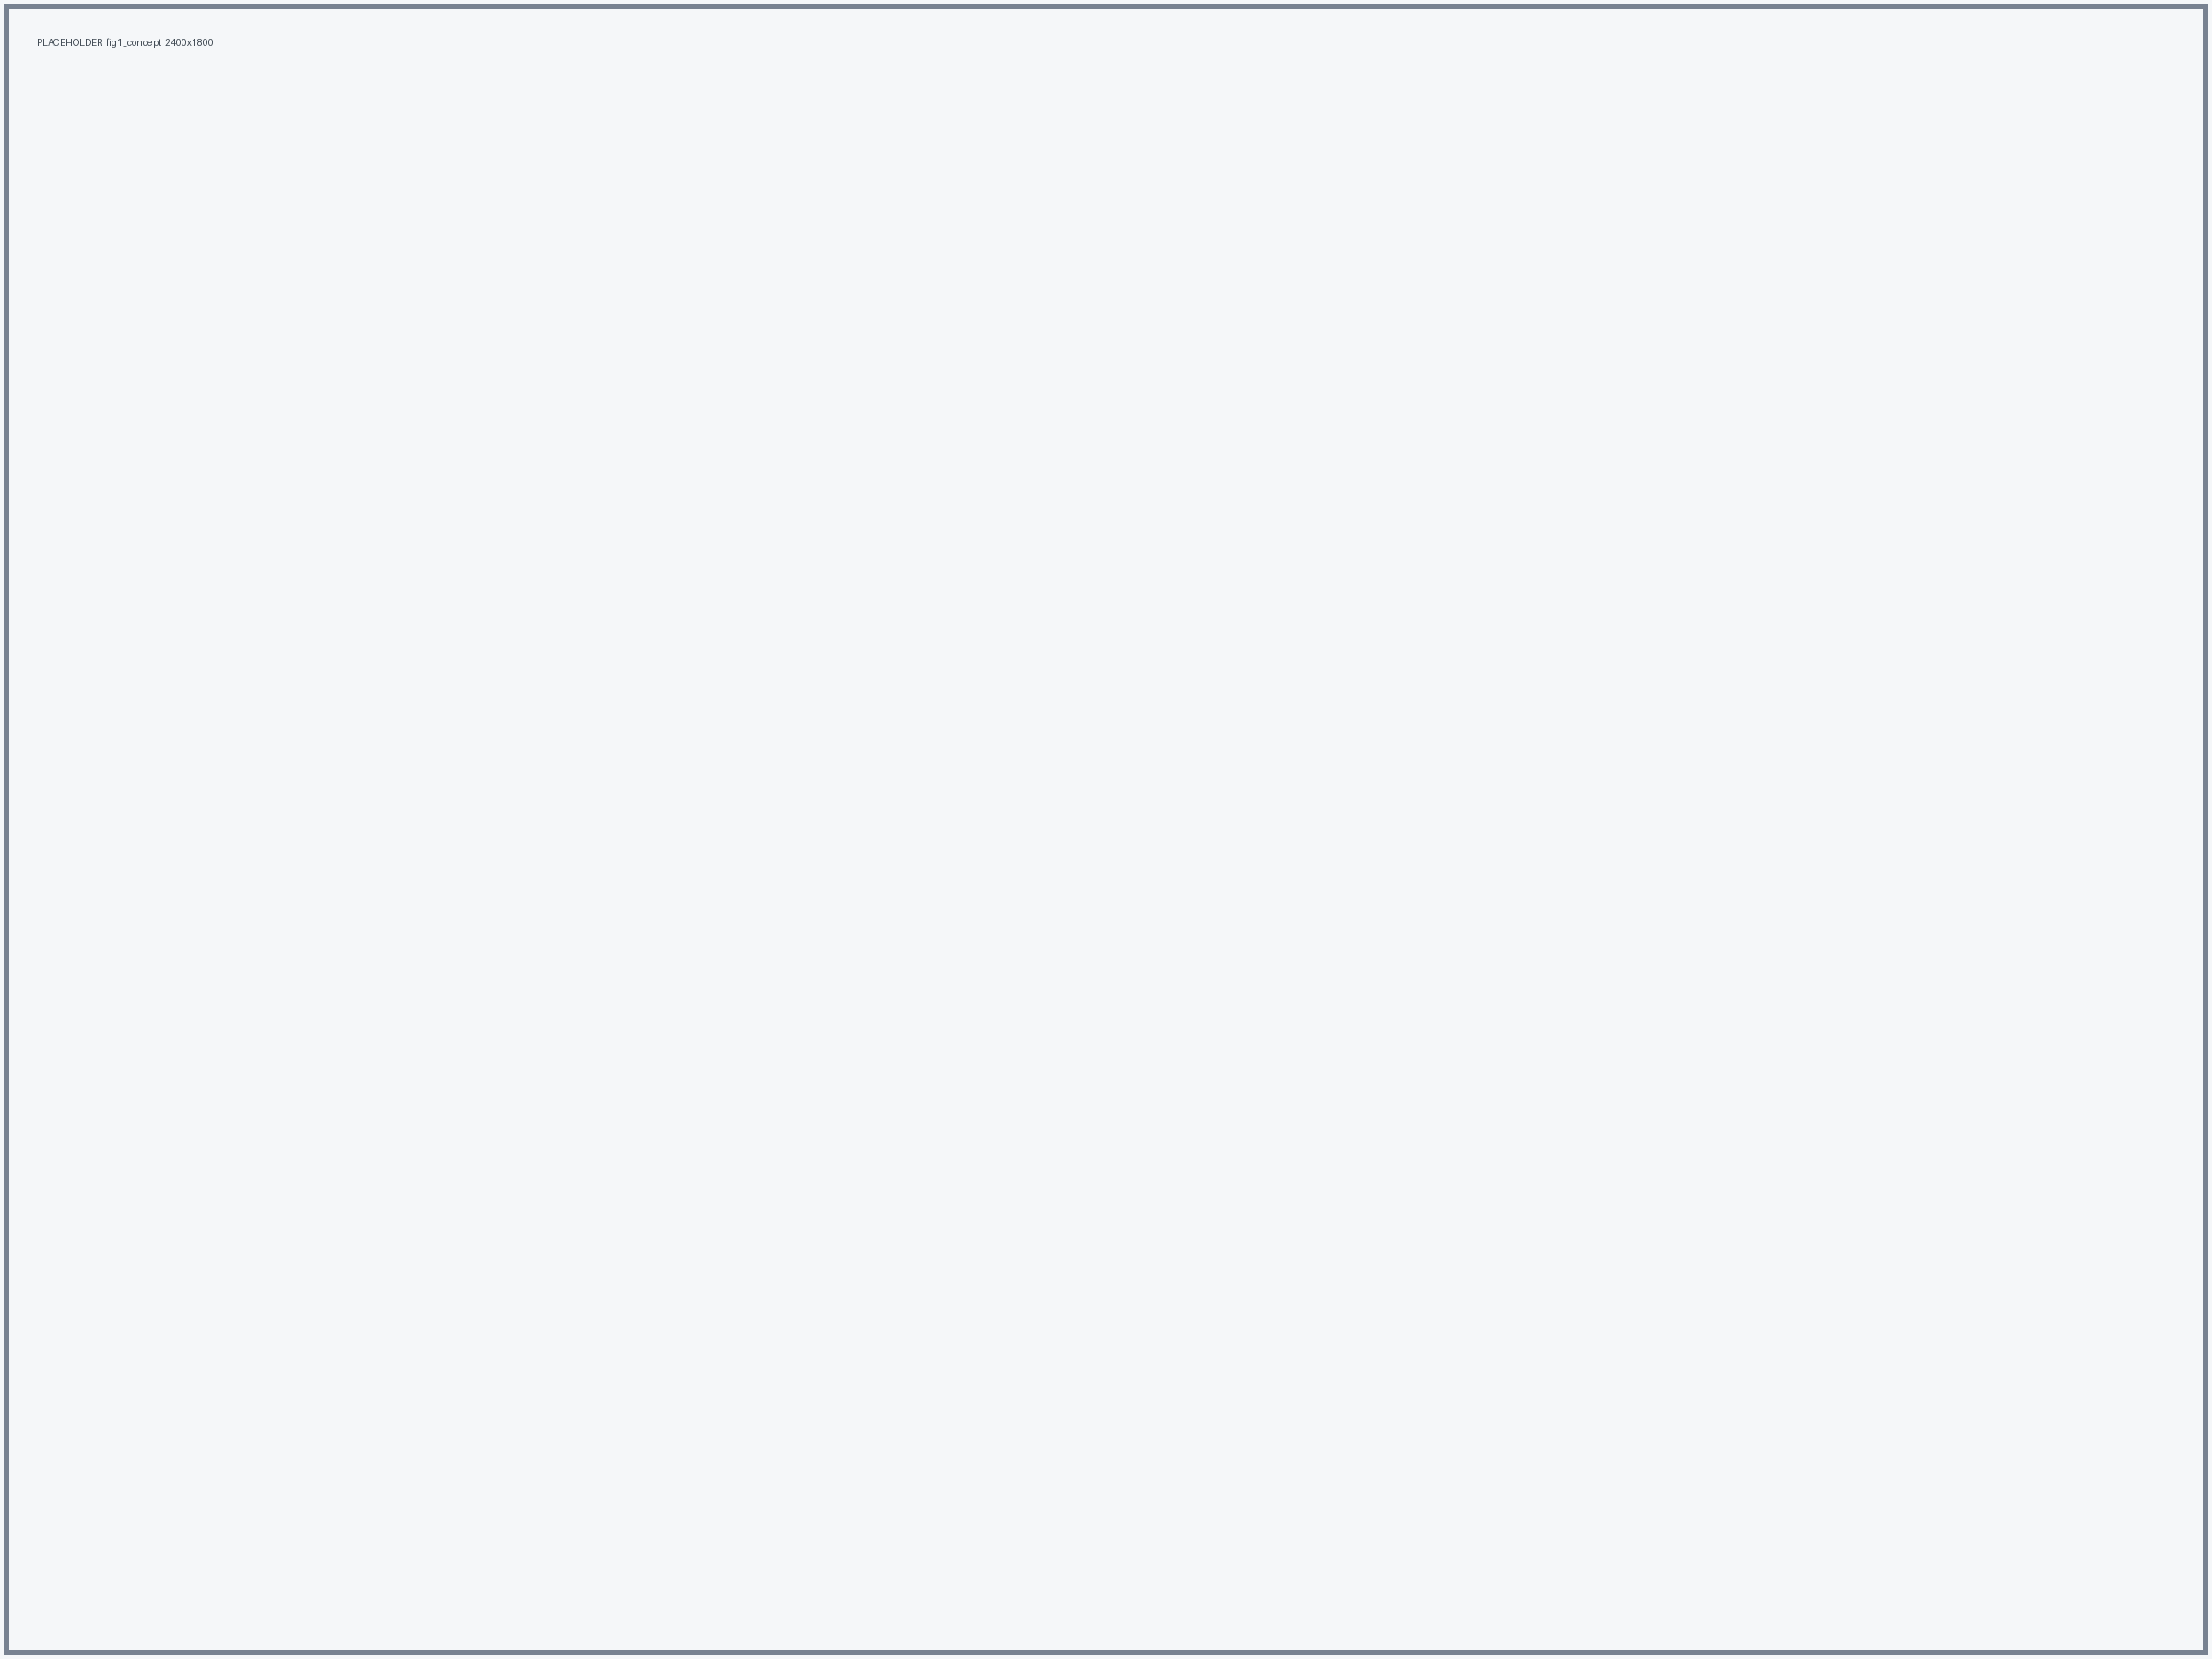
\includegraphics[width=80mm]{fig1_concept.png}
\caption{Engagement concept. A suicide USV swarm converges on the mothership
         from several bearings, while a smaller number of slower defending USVs
         close the approach corridors in advance with capture nets}
\label{fig:concept}
\end{figure}

방어정은 적선보다 느리므로 추격으로 따라잡을 수 없고, 대신 적선이 지나갈 접근 회랑을
앞질러 그물벽으로 차단한다(Fig.~\ref{fig:concept}).

다중 무인수상정의 협력 기동은 꾸준히 연구되어 왔고(Liu et al., 2016), 최근에는 다중
에이전트 강화학습으로 회피 표적을 협조 포위하는 정책을 학습한 사례도 보고되었다(Zhang
et al., 2025). 다만 추격·포위는 방어측 속력 우세를 전제하는 경우가 많다. 본 연구는
방어정이 더 느린 상황에서 추격의 방식 대신 예상 접근로를 사전에 차단한다는 점에서 구분된다.

방어의 성패는 유한한 자원을 어느 적 무리에 배정할 것인가와, 배정된 적을 어떻게 처리할
것인가에 달린다. 전자는 적의 접근 양상을 예측할 수 없어 상황에 따른 유연한 판단을 요구하고, 후자는 여러 방어정이 서로의 경로를 고려하는 협조 기동을 요구한다.
이 때 대규모 언어모델(Large Language Model, LLM)을 통해 알고리즘의 배정 방식보다 유연한 판단을 구현하고자 한다.
하지만 대규모 언어모델은 응답주기의 지연과 산술적 능력으로는 한계가 존재하여 해당 모델을 표적 아군 할당의 문제에만 국한하여 접목하였다.

%-------------------------------------------------- 그림 2 (양단 걸침)
% 배치 주의: figure* 는 선언된 페이지에는 놓이지 못하고 반드시 그 다음 페이지 이후의
%   단 상단으로 넘어간다. 2쪽 상단에 오게 하려면 1쪽이 조판되는 이 위치(서론 끝머리)에
%   선언되어 있어야 한다. 아래로 옮기면 3쪽으로 밀린다.
\begin{figure*}[t]
\centering
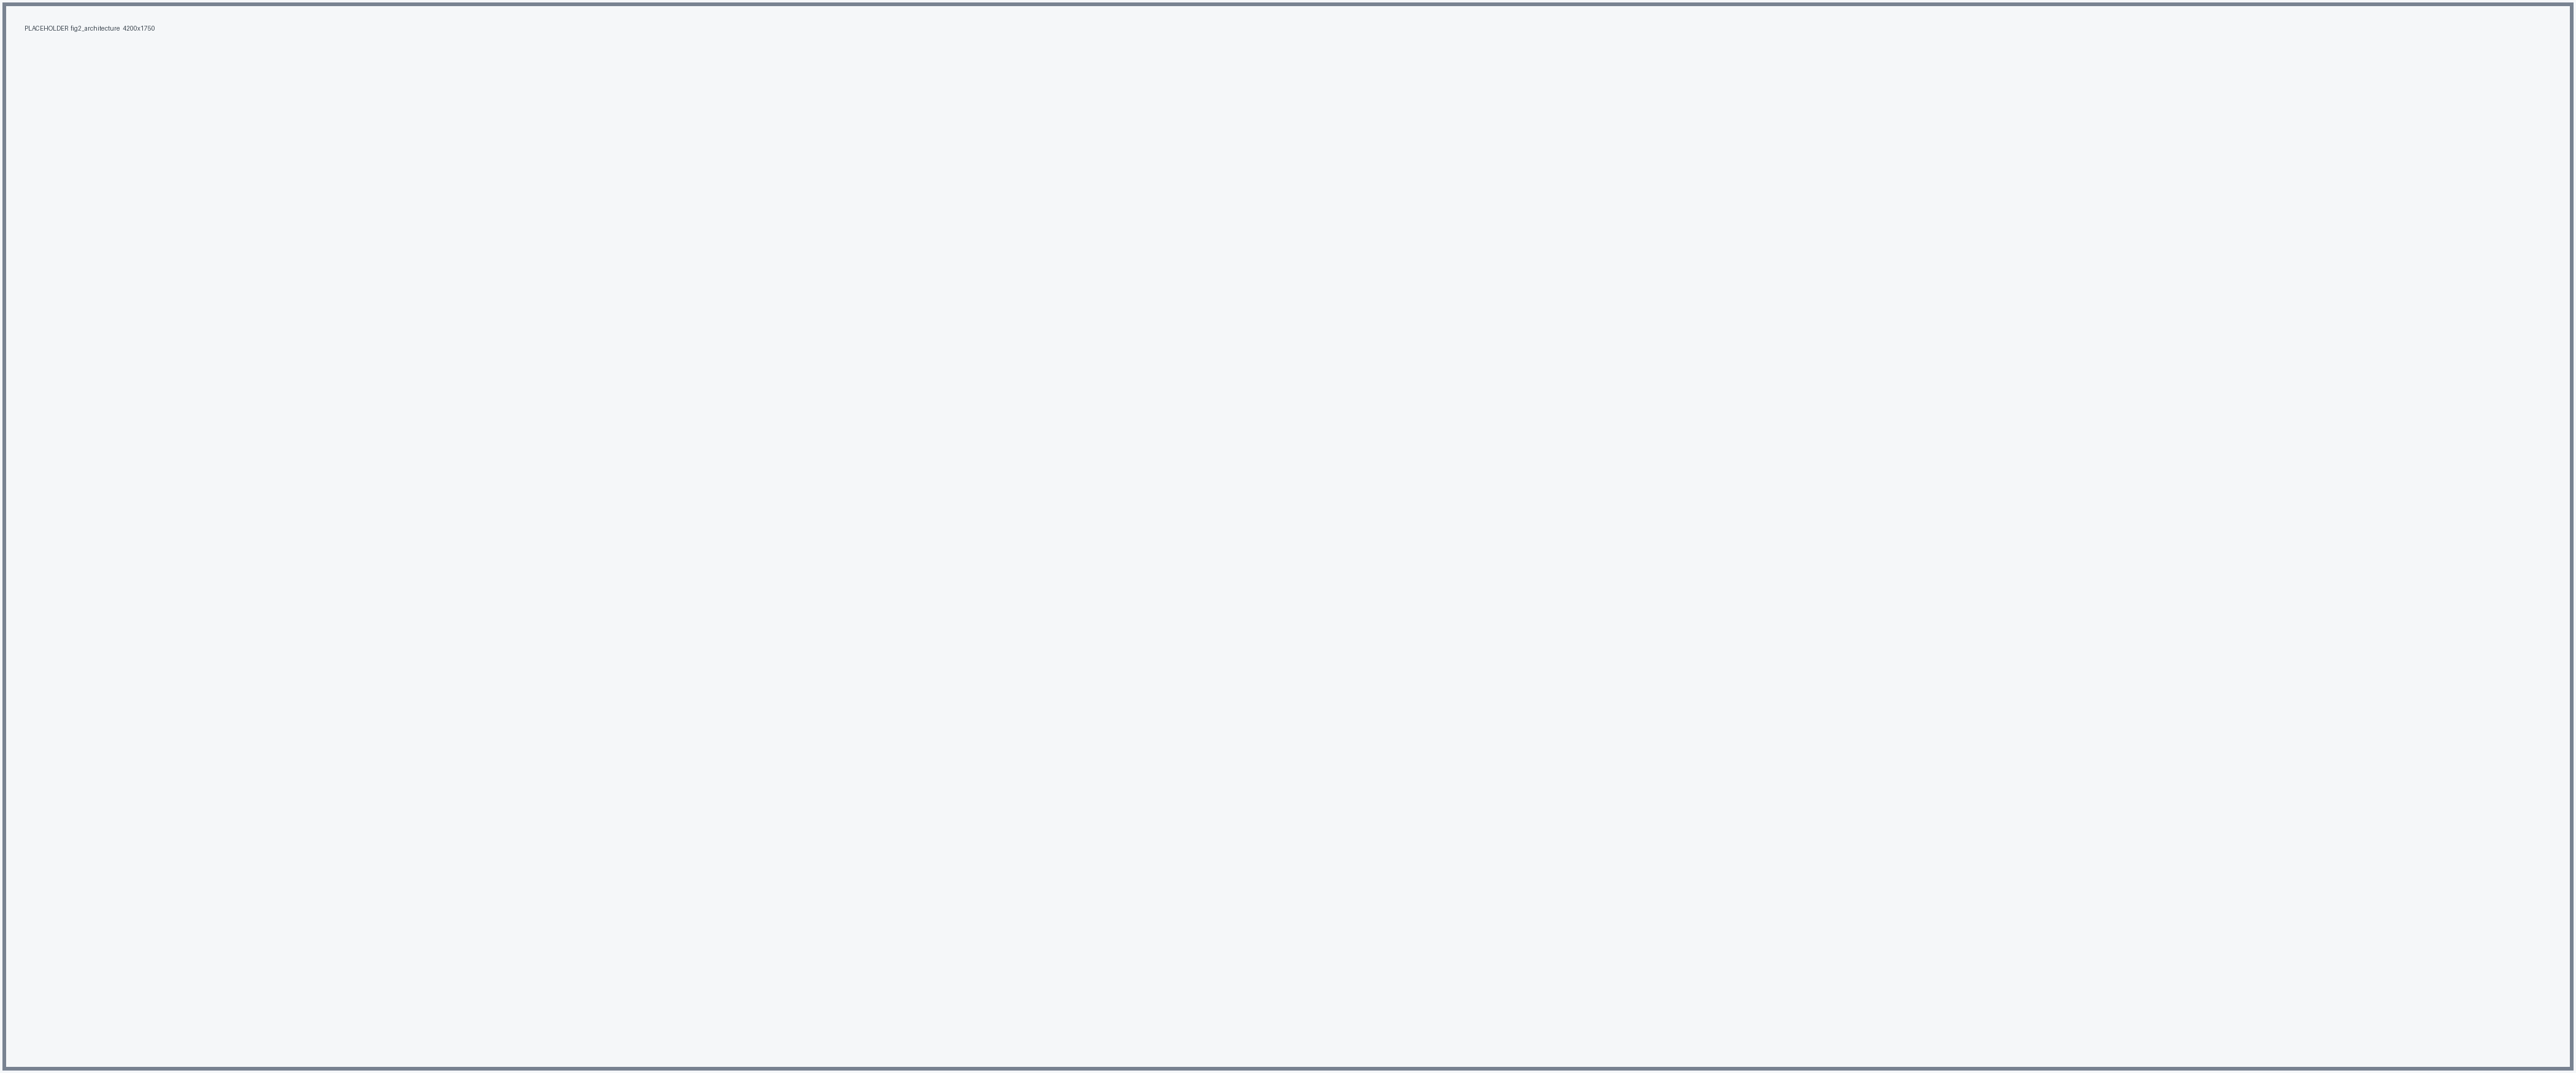
\includegraphics[width=0.92\textwidth]{fig2_architecture.png}
\caption{Two-layer defense system and its asynchronous decision cycles. The LLM
         commander turns the preprocessed battlefield state into a per-vessel
         assignment and hold decisions on a slow cycle; between successive
         replans the maneuver layer turns the rasterized battlefield image into
         a score map, picks waypoints on it, and lays nets along the segments
         joining them. The commander is called asynchronously, so its response
         latency does not stall the control loop}
\label{fig:architecture}
\end{figure*}

제안하는 체계는 이 두 요구를 각각 담당하는 두 계층으로 분리한다(Fig.~\ref{fig:architecture}). LLM
지휘관이 느린 주기로 적선별 담당 무리와 대기 방어정을 확정하면, 강화학습 정책이 전장을 담은
격자 지도로부터 배정된 적선을 포획하기 위해 그물을 투하할 위치를 선택한다. LLM 재계획 주기
사이에 강화학습 루프를 배치하여 고수준 판단은 LLM이, 실시간성이 요구되는 저수준 경유점
결정은 학습된 정책이 담당한다.

%=============================================================================
\section{제안 방법}

\subsection{문제 설정}

% ※ 확인 필요: 그물벽 최대 길이가 본문은 150 m 인데, 실제 학습 체크포인트
%   (boatattack_sim/models/u-net_map.pt) 의 config 는 net_max_len = 450 m 이다
%   (docs/unet_model_deploy.md §1). 둘 중 어느 쪽이 이 논문의 설정인지 확정할 것.
%   Fig. 1 / Fig. 5 의 그물벽 길이 비례도 확정된 값에 맞춰야 한다.
중앙에 고가치 모선이 위치, 가장자리에서
적선 $M=10$척이 접근한다. 아군 방어정은 $P=3$척이며 각각 최대 길이 150 m의 그물벽
하나를 전개할 수 있다(Fig.~\ref{fig:concept}). 성능 지표는 식 (1)의 포획률이다.

% fleqn 문서라 수식이 기본적으로 왼쪽 정렬된다. 이 식만 폭을 재어 단 가운데로 밀었다.
% (\columnwidth 짜리 상자에 담으면 식 번호가 같은 줄에 못 들어가 아래로 밀려난다.)
\newlength{\snakeqw}
\newcommand{\CaptureRateEq}{%
  \mathrm{Capture\ Rate}=\frac{N_\mathrm{cap}}{N_\mathrm{cap}+N_\mathrm{brc}}}
\settowidth{\snakeqw}{$\displaystyle\CaptureRateEq$}
\begin{equation}
\hspace*{\dimexpr(\columnwidth-\snakeqw)/2-\mathindent\relax}\CaptureRateEq
\end{equation}

여기서 $N_\mathrm{cap}$과 $N_\mathrm{brc}$는 각각 포획된 적선 수와 돌파한 적선 수이다.

\subsection{전략 계층: LLM 지휘관}

LLM에게 들어가는 정보는 좌표 원시 데이터 대신 기하량이 미리 계산된 형태로 직렬화되어 상황 판단을 위하여 해야할 계산을 미리 수행한 후 정보를 제공한다. 각 적
무리의 요격점까지의 이동거리와 선회량, 모선 기준 방위, 설치된 그물에 의한 접근로 차단
여부 등이 여기에 포함된다. 

출력은 구조적 출력(structured output)으로 강제되며(OpenAI, 2026), 판단 근거·무리별
배정·대기 목록 형태의 출력을 갖는다. 판단 근거를 사전에 먼저 출력하게 함으로 배정을 위한 판단을 할 때 사용자의 기준으로 설명 가능한 판단을 하게 한다. 해당 모델의 호출은 비동기로 이루어지며 그동안
경유점 생성및 추종은 이어서 진행이 되어 대규모 언어모델의 응답 지연이 제어 주기를 막지 않는다.

%-------------------------------------------------- 그림 3 (단단)
\begin{figure}[H]
\centering
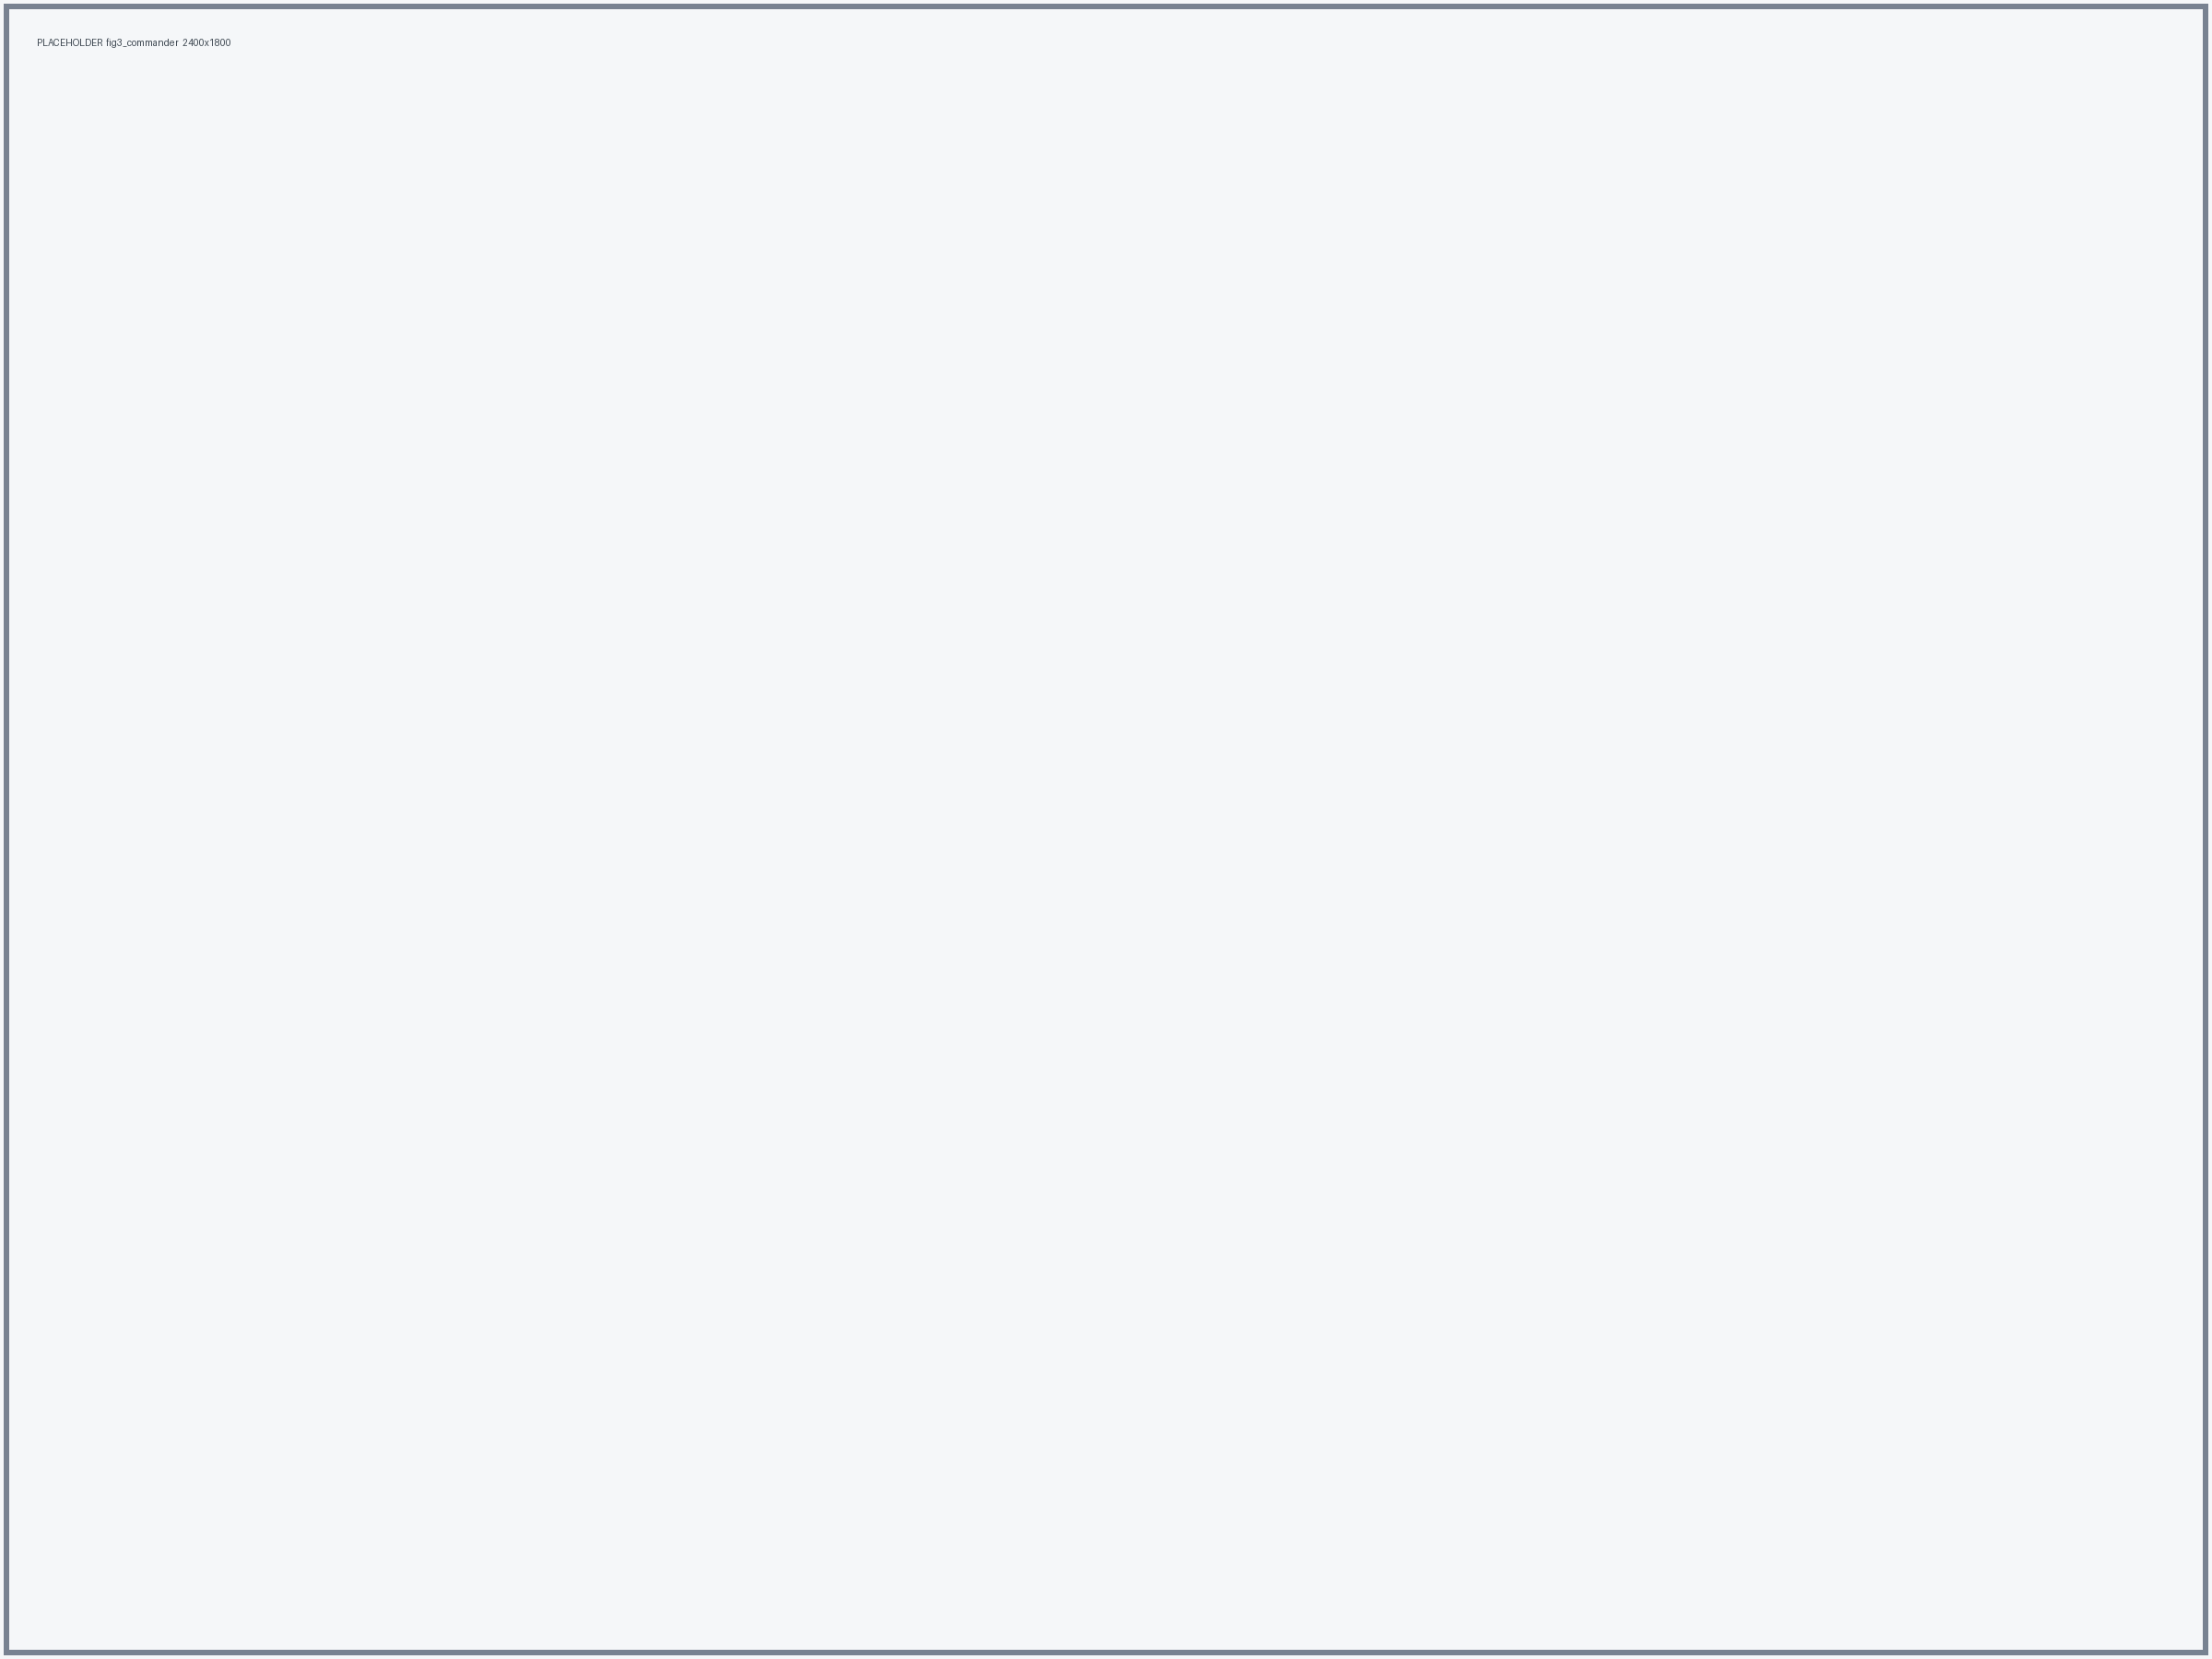
\includegraphics[width=80mm]{fig3_commander.png}
\caption{Commander layer. Precomputed geometric quantities are serialized into
         a table, the response is constrained to a fixed field order in which
         the rationale precedes the assignment, and the resulting assignment
         fixes each vessel's intercept point and the corridor of candidate
         cells around it}
\label{fig:commander}
\end{figure}

배정이 확정되면 각 방어정의 요격점이 정해지고, 그 요격점을 중심으로 하위 계층이 그물을
놓을 수 있는 후보 영역이 함께 결정된다(Fig.~\ref{fig:commander}). 즉 배정은 기동 계층의
선행 조건이며, 배정이 바뀌면 후보 영역 자체가 바뀐다.


\subsection{기동 계층: 점수맵 기반 좌표 선택 정책}

기동 계층의 입력은 좌표 목록이 아니라 모선을 중앙에 두고 전장을 일정 간격의 격자로 나눈 다채널 격자 지도이다. 적선과 아군의
위치·진행 방향, 위협도, 이미 설치된 그물, 모선과 요격 환형, 그리고 자기 자신과 배정된
요격점이 각각 하나의 채널로 그려진다. 목록 대신 격자 지도를 입력으로 쓰면 교전 중 적선의 수가
늘거나 줄어도 입력의 형태가 달라지지 않고, 적선을 어떤 순서로 넣었는지에 따라 결과가
바뀌지도 않는다. 다만 합성곱만으로는 물체가 지도의 어디에 있는지가 흐려지므로, 각 칸의
좌표를 담은 채널을 함께 넣어 절대 위치를 보존한다(Liu et al., 2018). 이렇게 구성된 관측은
전역 공통 채널과 방어정별 채널, 좌표 채널의 세 묶음으로 이루어진 하나의 다채널 영상이 된다
(Fig.~\ref{fig:observation}).

%-------------------------------------------------- 그림 4 (단단)
\begin{figure}[H]
\centering
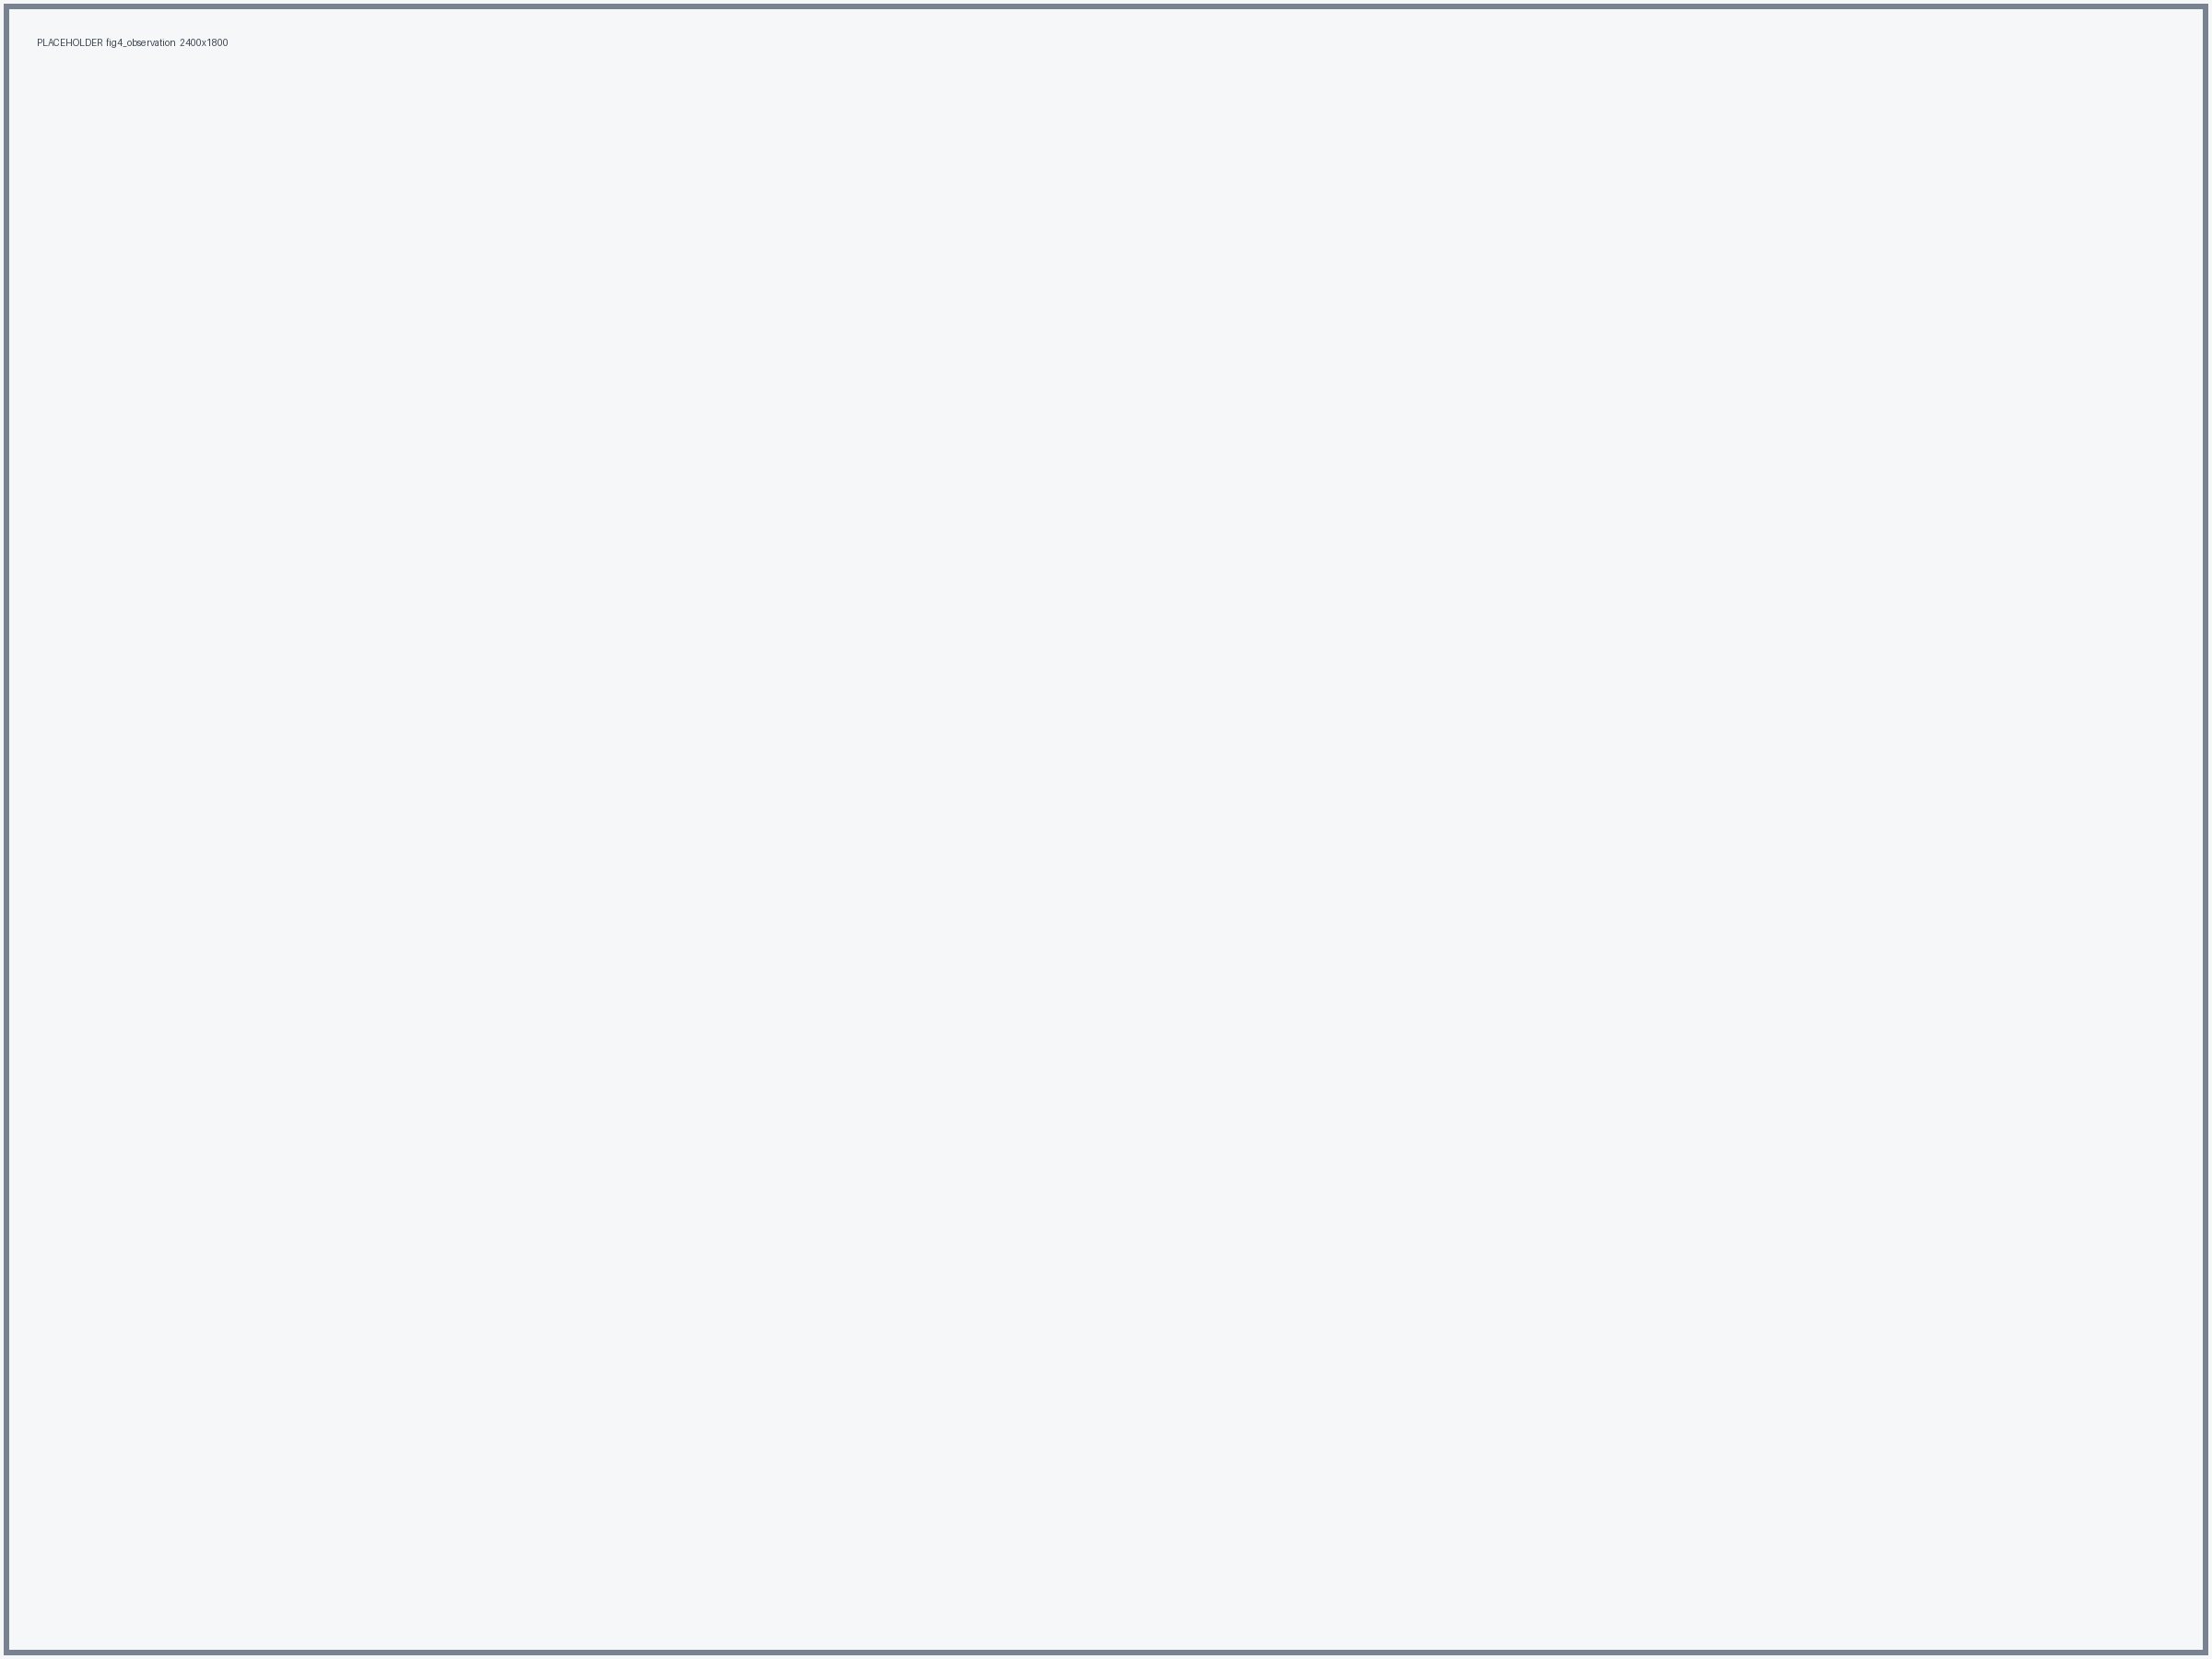
\includegraphics[width=80mm]{fig4_observation.png}
\caption{Rasterized multi-channel observation. The battlefield is quantized
         onto a fixed grid centred on the mothership and drawn into global,
         per-vessel, and coordinate channels, so that the input shape stays
         fixed as the number of targets changes}
\label{fig:observation}
\end{figure}

이 격자 지도는 U-Net 구조의 합성곱 신경망을 지나 입력과 같은 해상도의 점수맵으로
변환된다(Ronneberger et al., 2015). 점수맵의 각 칸은 그 지점에 그물을 놓는 것이 얼마나
좋은지를 나타내며, 방어정은 자기 상태로부터 만든 질의 벡터와 칸 특징의 내적으로 이 점수를
얻는다. 각 방어정은 배정된 적군 주변으로 제한된 유효 영역 안에서 점수가 높은 칸 2개를
순차적으로 선택하되, 먼저 고른 칸의 특징을 질의에 반영하여 두 점이 서로를 알고 뽑히도록
한다. 선택된 두 좌표를 잇는 구간이 그물을 설치할 하나의 경로가 되고, 방어정은 그 경로를
이동하며 그물을 투하한다(Fig.~\ref{fig:policy}). 연속 경유점을 회귀시키는 대신 점수맵
위의 칸을 지목함으로써 행동공간을 규제하고 결정된 경유점의 위치를 고정하여 안정적인 기동을
할 수 있도록 한다.

%-------------------------------------------------- 그림 5 (양단 걸침)
% figure* 는 선언된 페이지 다음 페이지의 단 상단으로 넘어간다. 이 절에서 선언해야
%   Fig. 4(관측)보다 늦게 번호가 매겨지면서 다음 쪽 상단에 놓인다.
\begin{figure*}[t]
\centering
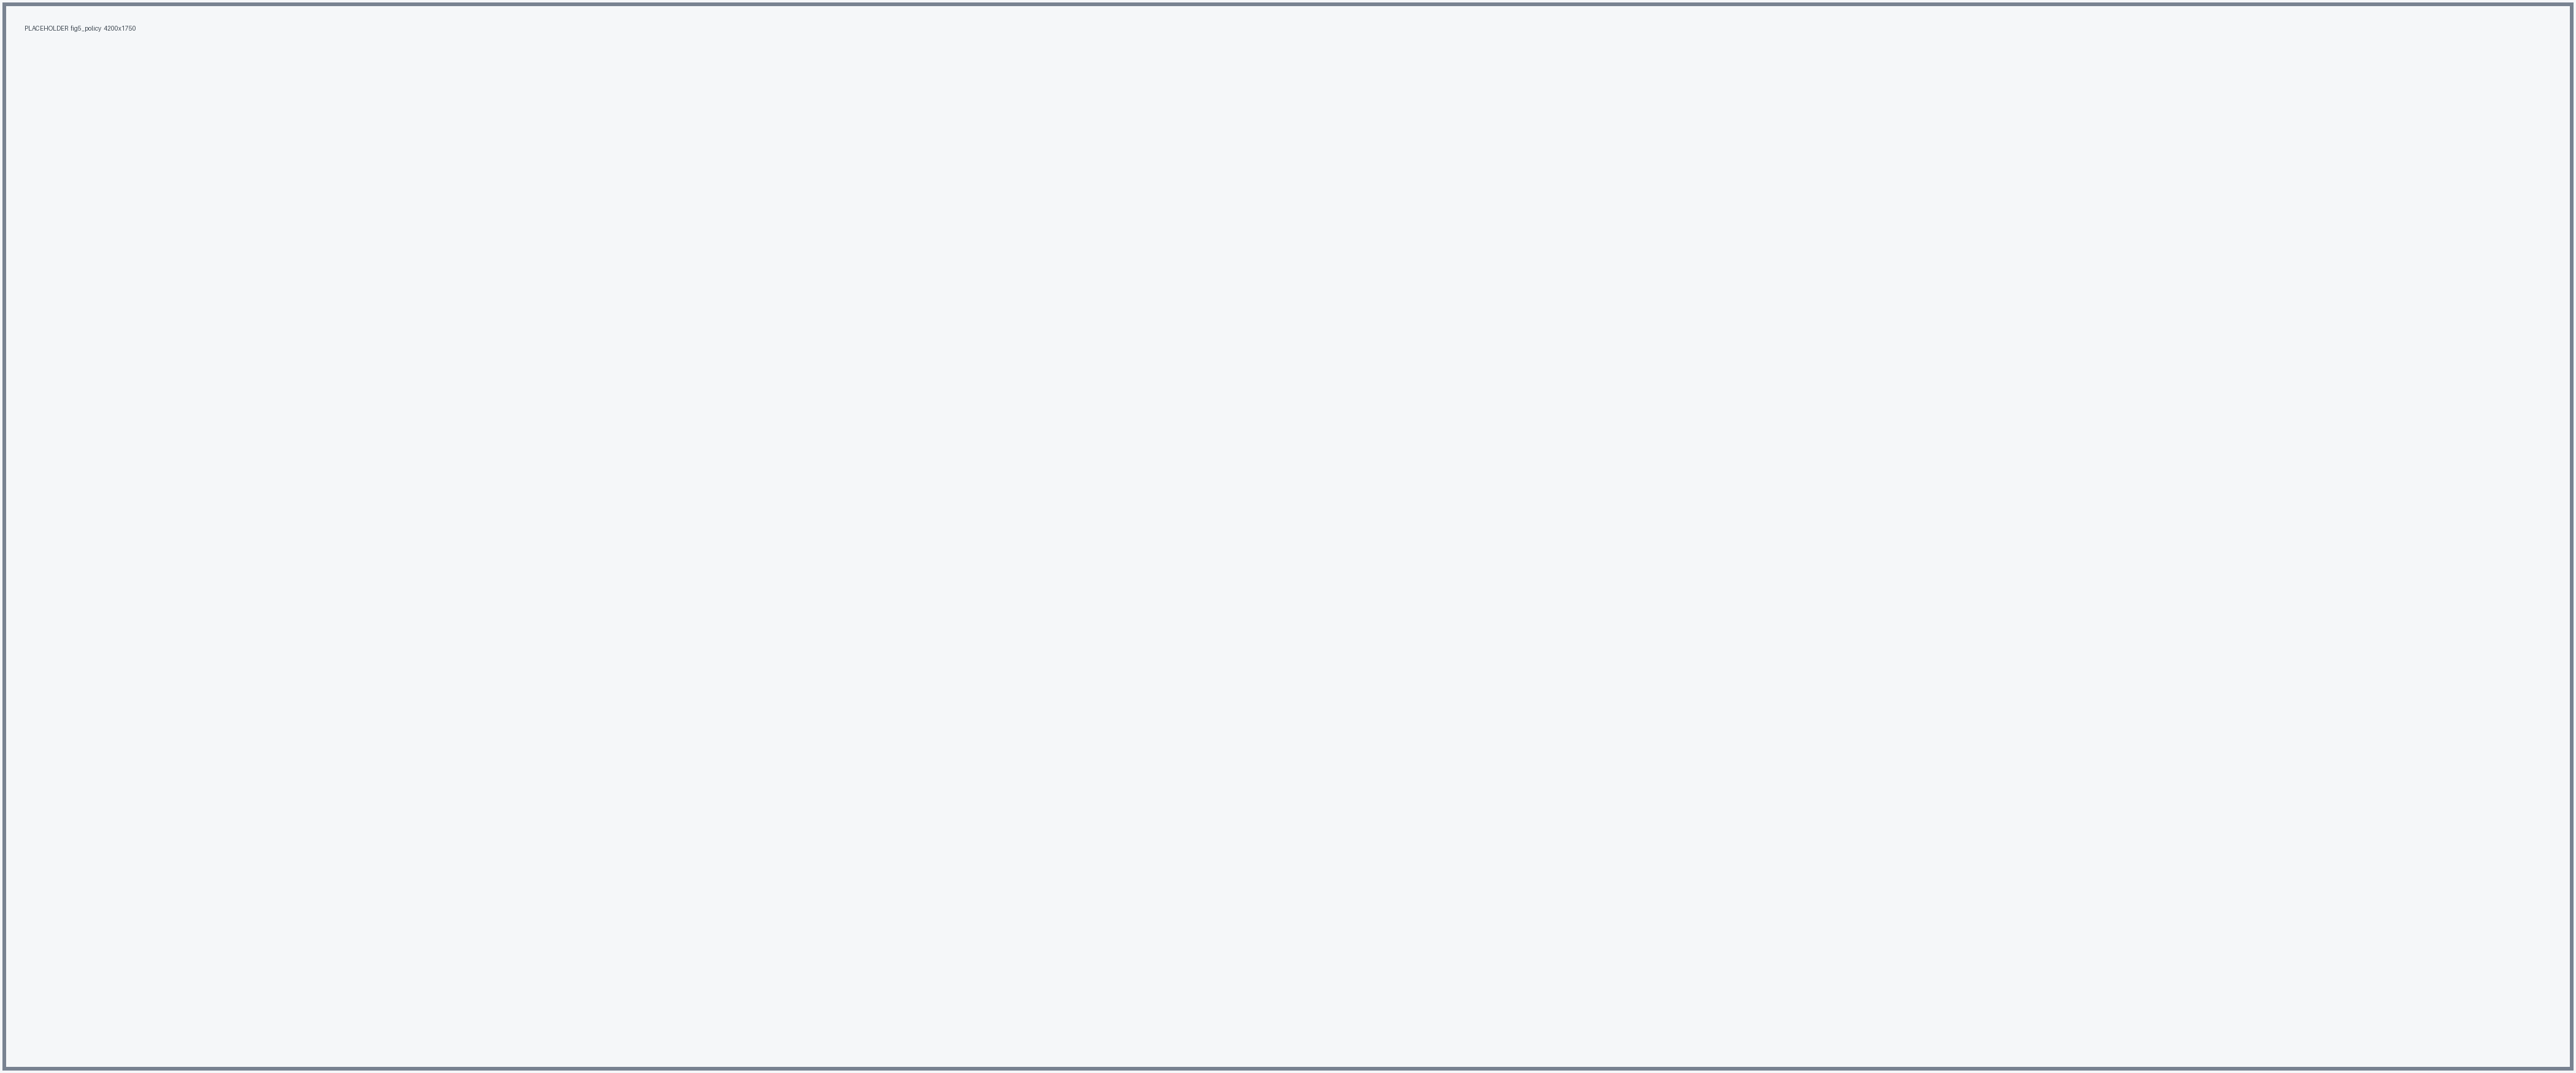
\includegraphics[width=0.94\textwidth]{fig5_policy.png}
\caption{Score-map maneuver policy. The multi-channel observation passes through
         a U-Net that preserves the input resolution; the inner product between
         a query built from the vessel's own state and the per-cell features
         yields a score over the sea surface. Outside the valid region the score
         is masked away, two cells are picked in sequence with the first pick
         fed back into the query, and the segment joining them is laid as a net
         wall}
\label{fig:policy}
\end{figure*}

학습은 가치함수를 따로 두지 않는 그룹 상대 정책 최적화(GRPO)를 다중 방어정 상황에 맞게
변형하여 수행하였다(Shao et al., 2024)(Fig.~\ref{fig:grpo}). 매 결정 시점에서 정책으로부터 여러 개의 후보 행동을
뽑고, 각 후보를 시뮬레이터에서 일정 구간 진행시켜 팀 보상을 얻은 뒤, 이 후보들끼리의 상대
비교로 이득을 산정한다. 어떤 선택이 더 나았는지를 실제 결과로 직접 비교하므로 별도의
가치망이 필요하지 않다. 다만 팀 보상을 모든 방어정이 그대로 나누어 가지면 개별 기여를
가릴 수 없으므로, 한 척의 행동만 바꾸고 나머지는 고정한 채 평가하여 그 차이를 해당
방어정의 몫으로 돌린다. 후보 가운데 하나는 휴리스틱이 내는 행동으로 채워 초기 학습의
출발점을 확보하였다. 보상은 포획, 돌파, 아군의 그물 접촉을 지배 항으로 하고, 위협
근접도에 대한 퍼텐셜 항을 두어 최적 정책을 보존하는 형태로 구현하였다(Ng et al., 1999).

%-------------------------------------------------- 그림 6 (단단)
\begin{figure}[H]
\centering
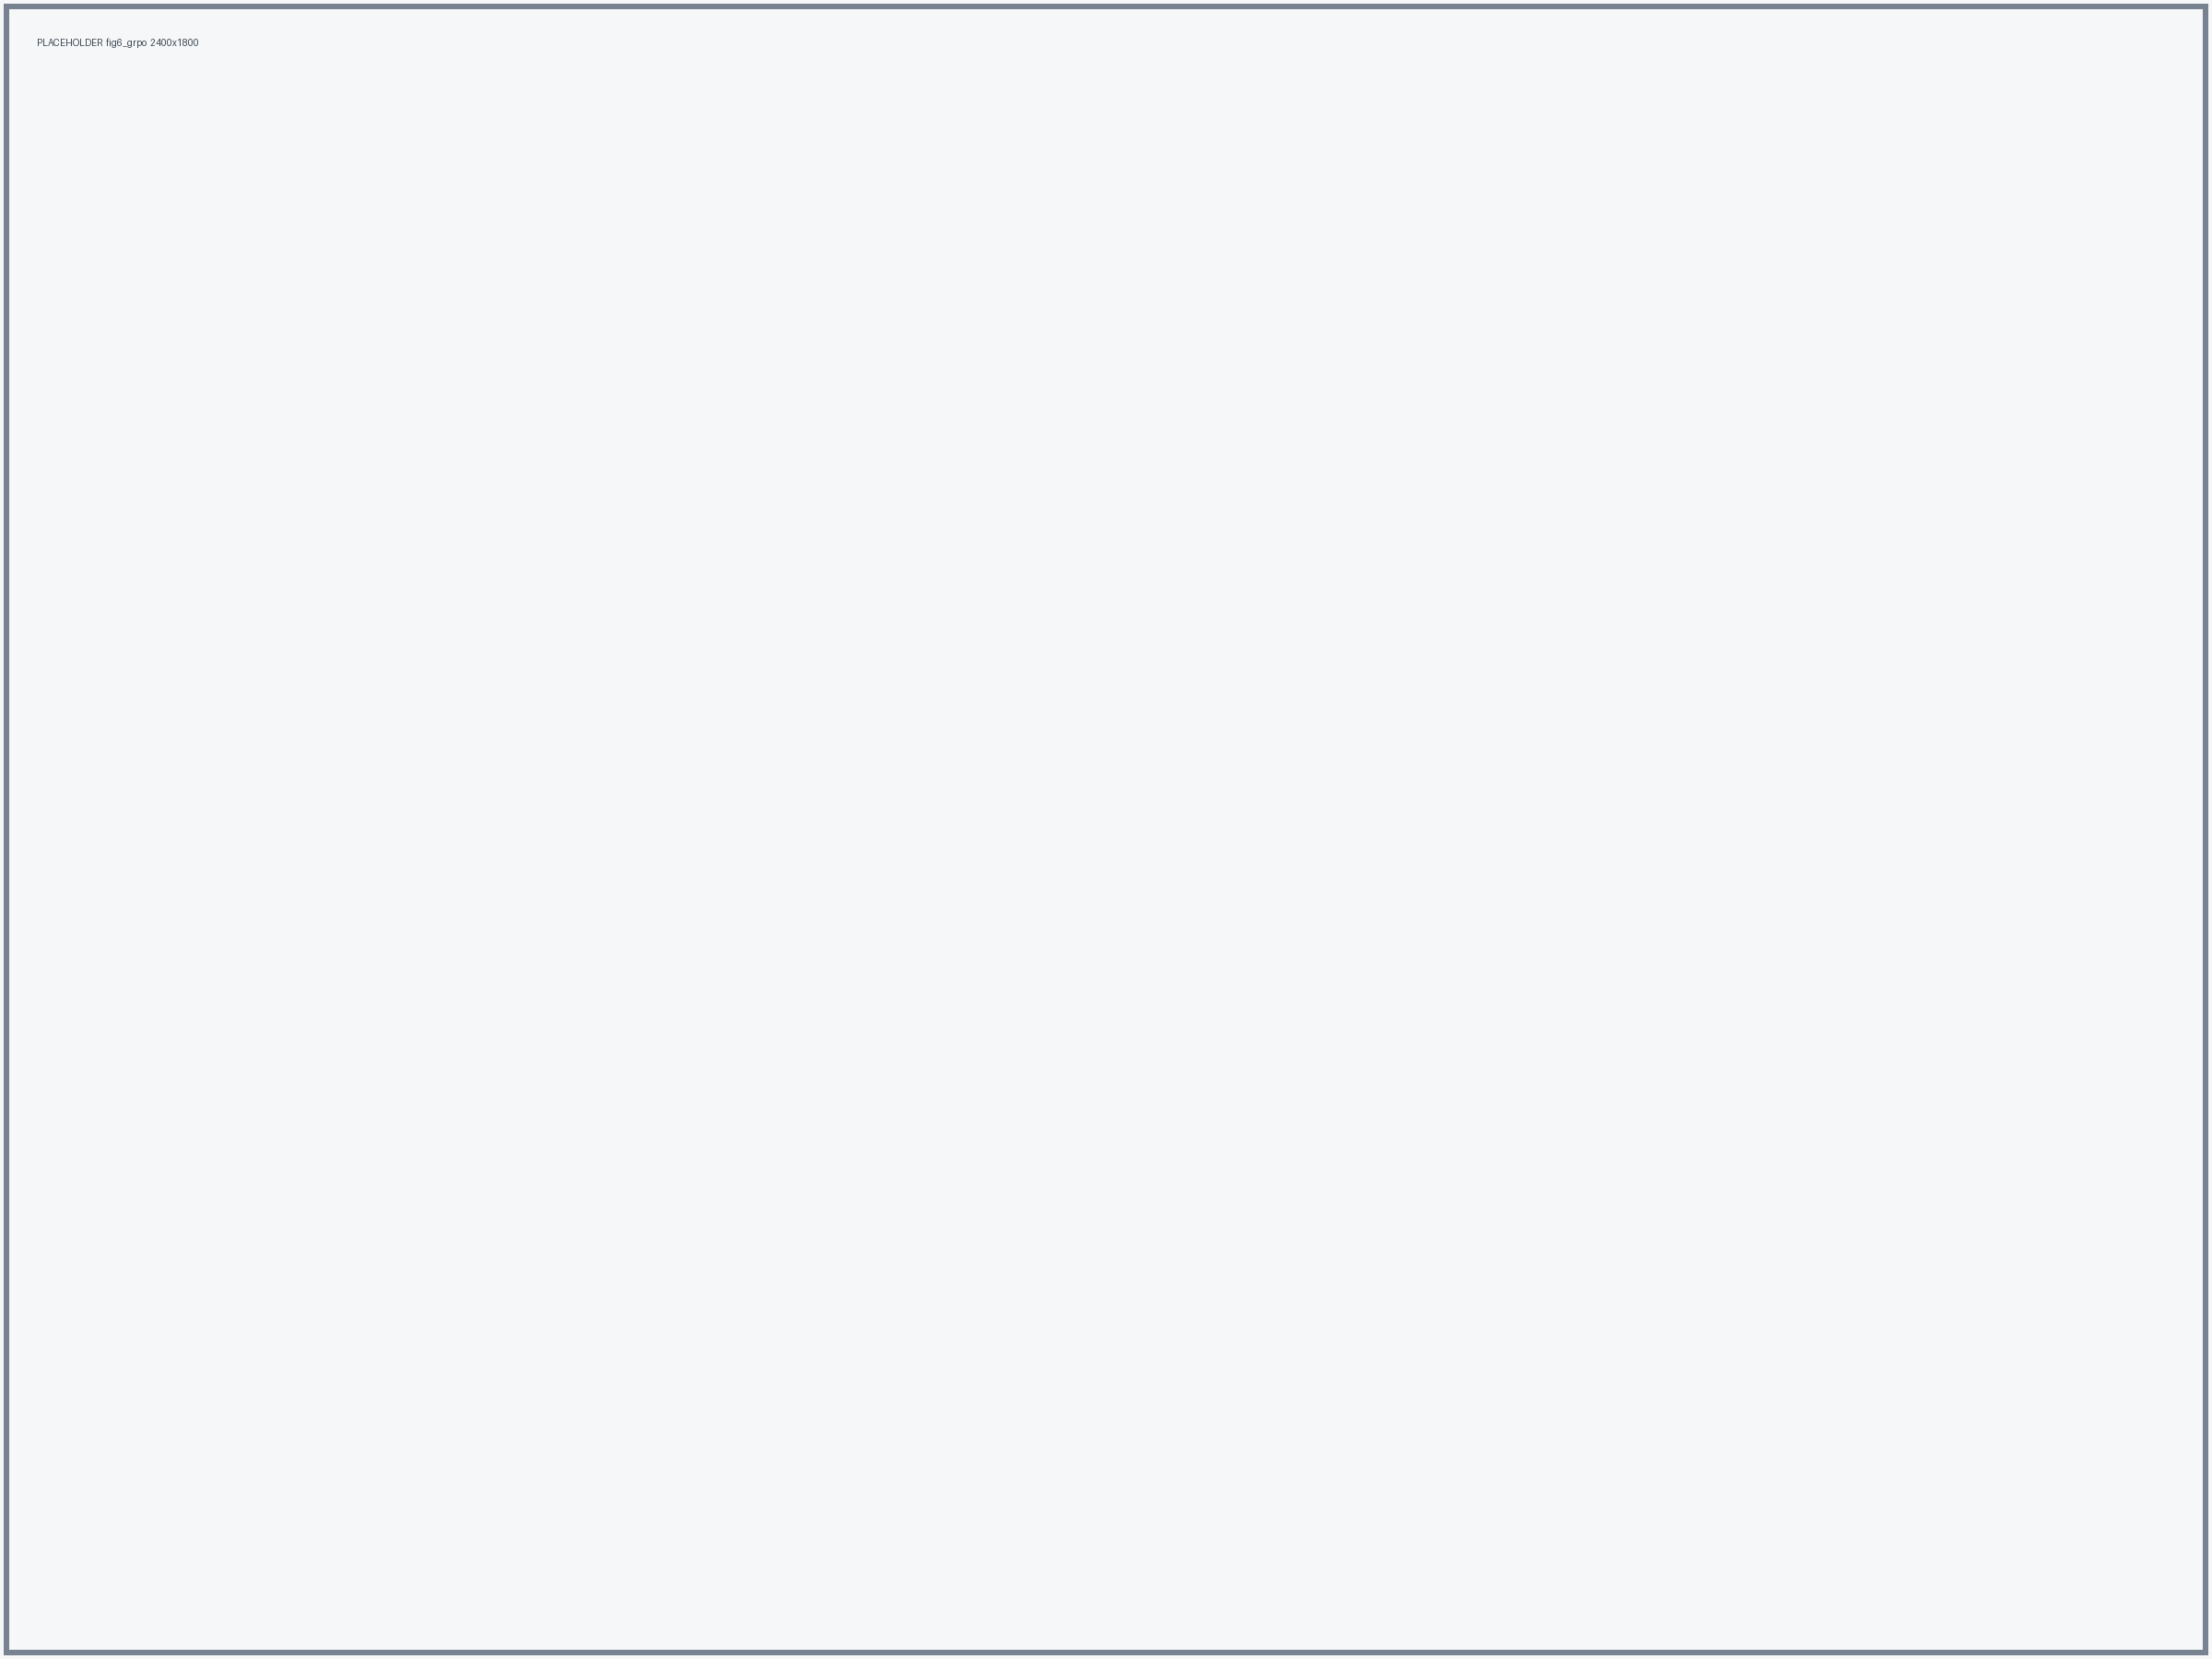
\includegraphics[width=80mm]{fig6_grpo.png}
\caption{Group-relative training with per-vessel counterfactual credit.
         Candidate actions sampled at one decision point are advanced through
         the simulator over a common window; the resulting team rewards are
         compared against the group mean, and perturbing a single vessel while
         holding the others fixed isolates that vessel's contribution}
\label{fig:grpo}
\end{figure}

%=============================================================================
\section{결 론}

본 연구는 자폭 무인수상정 군집에 대한 대응으로 저비용 그물을 이용한 물리적 포획을
채택하고, 이를 판단 주기가 서로 다른 계층으로 분리하여 구성하였다. 상위에서는 LLM
지휘관이 기하량이 미리 계산된 전장 상태를 받아 아군별 담당 무리와 대기 방어정을 결정하고,
하위에서는 강화학습 정책이 그 배정 아래에서 전장 격자 지도로부터 그물벽을 놓을 좌표를
선택한다. LLM 재계획 주기 사이에 강화학습 결정 루프를 배치함으로써, 응답 지연을 수반하는
고수준 판단과 매 스텝 갱신되는 저수준 기동이 서로를 막지 않도록 하였다.

배정은 조합 최적화의 보정 없이 언어모델의 판단만으로 확정된다. 최소비용 매칭과 같은
후처리를 덧붙이면 최종 배정이 결국 비용 함수의 산물이 되어 지휘관의 전술적 의도가
가려지므로, 언어모델이 내린 결정을 하위 계층이 그대로 소비하는 구조를 택하였다. 이를
가능하게 한 것은 출력 형식을 미리 선언하는 구조적 출력과, 판단 근거를 결정보다 먼저
생성시키는 항목 배치이다.

기동 계층에서는 전장을 다채널 격자 지도로 인코딩하고, 합성곱 신경망이 낸 점수맵 위에서
경유점을 지목하게 하여 행동공간을 규제하였다. 목록 대신 지도를 입력으로 삼으므로 교전 중
적선의 수가 달라져도 입력의 형태가 유지되며, 선택된 경유점의 위치가 고정되므로 기동이
안정적으로 유지된다. 여기에 후보 행동을 실제로 진행시켜 서로 비교하는 학습 방식을 결합하여
별도의 가치망 없이도 방어정별 기여를 구분한 학습이 성립한다.

이로써 응답 지연을 감수하는 언어모델의 전술 판단과 매 스텝의 강화학습 기동이 서로를
기다리지 않고 병렬로 추론을 진행하며, 담당 무리의 배정에서 그물 투하까지 이어지는 방어체계를 구성하였다.


%=============================================================================
\begin{snakreferences}
% 저자 알파벳순. 본문에서 1회 이상 인용된 문헌만 기재한다(SNAK 지침).
% 요약본 분량에 맞추어 12편으로 축약하였다(2026-08-11). 관련 연구 장을 되살릴 경우
% Ahn / Huang / Kool / Liang / Oliehoek / Schulman(2016) / Vaswani 항목을 함께 복원할 것.
% 전 항목 원문 대조 완료(2026-08-12). 조합 최적화 계층을 삭제하면서 Kuhn(1955)은
% 인용처가 사라져 제외하였다. 되살릴 경우 함께 복원할 것.

Ahuja, R.K. Kumar, A. Jha, K.C. \& Orlin, J.B., 2007. Exact and Heuristic
Algorithms for the Weapon-Target Assignment Problem. \textit{Operations
Research}, 55(6), pp.1136-1146.

Liu, R. Lehman, J. Molino, P. Petroski Such, F. Frank, E. Sergeev, A. \&
Yosinski, J., 2018. An Intriguing Failing of Convolutional Neural Networks and
the CoordConv Solution. \textit{Advances in Neural Information Processing
Systems 31 (NeurIPS 2018)}, Montreal, Canada, 2-8 December 2018.

Liu, Z. Zhang, Y. Yu, X. \& Yuan, C., 2016. Unmanned surface vehicles: An
overview of developments and challenges. \textit{Annual Reviews in Control}, 41,
pp.71-93.

Ng, A.Y. Harada, D. \& Russell, S., 1999. Policy Invariance Under Reward
Transformations: Theory and Application to Reward Shaping. \textit{Proceedings
of the 16th International Conference on Machine Learning (ICML)}, Bled,
Slovenia, 27-30 June 1999, pp.278-287.

OpenAI, 2026. \textit{Function calling}. [Online] Available at:
\texttt{https://developers.openai.com/api/docs/guides/function-calling}
[Accessed 9 August 2026].

Ronneberger, O. Fischer, P. \& Brox, T., 2015. U-Net: Convolutional Networks for
Biomedical Image Segmentation. \textit{Medical Image Computing and
Computer-Assisted Intervention (MICCAI 2015)}, Munich, Germany,
5-9 October 2015, pp.234-241.

Rumbaugh, W., 2024. \textit{Cost and Value in Air and Missile Defense
Intercepts}. Washington, DC: Center for Strategic and International Studies
(CSIS) Commentary, 13 February 2024. [Online] Available at:
\texttt{https://www.csis.org/\allowbreak analysis/\allowbreak
cost-and-value-air-and-\allowbreak missile-defense-intercepts}
[Accessed 9 August 2026].

Shao, Z. Wang, P. Zhu, Q. Xu, R. Song, J. Bi, X. Zhang, H. Zhang, M. Li, Y.K.
Wu, Y. \& Guo, D., 2024. DeepSeekMath: Pushing the Limits of Mathematical
Reasoning in Open Language Models. \textit{arXiv preprint arXiv:2402.03300}.

Sutea, V., 2026. \textit{Fiber-optic drones have emerged as critical kit for
both Russia and Ukraine}. Atlantic Council UkraineAlert, 24 February 2026.
[Online] Available at: \texttt{https://www.atlanticcouncil.org/\allowbreak
blogs/ukrainealert/\allowbreak fiber-optics-drones-have-\allowbreak
emerged-as-critical-kit-\allowbreak for-both-russia-and-ukraine/}
[Accessed 12 August 2026].

Wang, J. Liu, Y. \& Song, H., 2021. Counter-Unmanned Aircraft System(s) (C-UAS):
State of the Art, Challenges, and Future Trends. \textit{IEEE Aerospace and
Electronic Systems Magazine}, 36(3), pp.4-29.

Zhang, C. Zeng, R. Lin, B. Zhang, Y. Xie, W. \& Zhang, W., 2025. Multi-USV
cooperative target encirclement through learning-based distributed transferable
policy and experimental validation. \textit{Ocean Engineering}, 318, 120124.

\end{snakreferences}

\end{document}
